\documentclass[12pt,a4paper]{article}

\usepackage{fontspec}
\IfFontExistsTF{Noto Serif}
  {\setmainfont{Noto Serif}}
  {\IfFontExistsTF{DejaVu Serif}{\setmainfont{DejaVu Serif}}{\setmainfont{Latin Modern Roman}}}
\IfFontExistsTF{Noto Sans}
  {\setsansfont{Noto Sans}}
  {\IfFontExistsTF{DejaVu Sans}{\setsansfont{DejaVu Sans}}{\setsansfont{Latin Modern Sans}}}
\IfFontExistsTF{Noto Sans Mono}
  {\setmonofont{Noto Sans Mono}}
  {\IfFontExistsTF{DejaVu Sans Mono}{\setmonofont{DejaVu Sans Mono}}{\setmonofont{Latin Modern Mono}}}

\usepackage[top=1.55cm,bottom=1.7cm,left=1.9cm,right=1.9cm]{geometry}
\usepackage{setspace}
\setstretch{1.06}
\usepackage{amsmath,amssymb}
\usepackage{graphicx}
\usepackage{booktabs}
\usepackage{tabularx}
\usepackage{float}
\usepackage{caption}
\captionsetup{font=small,labelfont=bf,skip=3pt}
\renewcommand{\figurename}{Hình}
\renewcommand{\tablename}{Bảng}
\renewcommand{\refname}{Tài liệu tham khảo}
\usepackage{titlesec}
\titleformat{\section}{\large\bfseries\sffamily}{\thesection.}{0.45em}{}
\titlespacing*{\section}{0pt}{7pt}{3pt}
\titleformat{\subsection}{\normalsize\bfseries\sffamily}{\thesubsection}{0.45em}{}
\titlespacing*{\subsection}{0pt}{5pt}{2pt}
\usepackage{enumitem}
\setlist{nosep,leftmargin=1.15em}
\usepackage{xcolor}
\usepackage{hyperref}
\hypersetup{colorlinks=true,linkcolor=blue!45!black,urlcolor=blue!45!black,citecolor=blue!45!black}
\usepackage{fancyhdr}
\pagestyle{fancy}
\fancyhf{}
\fancyfoot[C]{\thepage}
\renewcommand{\headrulewidth}{0pt}
\usepackage{microtype}

\newcommand{\University}{TRƯỜNG ĐẠI HỌC KHOA HỌC TỰ NHIÊN}
\newcommand{\Faculty}{KHOA TOÁN CƠ - TIN HỌC}
\newcommand{\StudentName}{Dương Quang Huy}
\newcommand{\StudentId}{23001524}
\newcommand{\Major}{Khoa học dữ liệu}
\newcommand{\Course}{68}
\newcommand{\Supervisor}{GS. Đỗ Minh Đức}
\newcommand{\ReportTitle}{PHÂN TÍCH VÀ DỰ BÁO CHUỖI THỜI GIAN LƯU LƯỢNG DÒNG CHẢY SÔNG COLORADO GIAI ĐOẠN 2010--2023}
\newcommand{\ReportPlaceYear}{Hà Nội, 2026}

% Sinh tự động bởi export_latex.py; không sửa tay.

\newcommand{\DatasetN}{5.113}
\newcommand{\DateMin}{2010/01/01}
\newcommand{\DateMax}{2023/12/31}
\newcommand{\QMean}{295{,}68}
\newcommand{\QStd}{99{,}32}
\newcommand{\QMin}{94{,}39}
\newcommand{\QMax}{457{,}49}
\newcommand{\QMedian}{334{,}40}
\newcommand{\QHigh}{417{,}23}
\newcommand{\NDaysHigh}{256}
\newcommand{\ShareHigh}{5{,}01}
\newcommand{\NEvents}{15}
\newcommand{\ZThreshold}{1{,}224}
\newcommand{\TrainOrigins}{3.615}
\newcommand{\ValOrigins}{725}
\newcommand{\TestOrigins}{724}
\newcommand{\RefitOrigins}{4.346}
\newcommand{\SeasonalStrength}{0{,}104}
\newcommand{\TrendStrength}{0{,}966}
\newcommand{\AcfYear}{-0{,}148}
\newcommand{\MonthlyMinMonth}{9}
\newcommand{\MonthlyMinValue}{292{,}32}
\newcommand{\MonthlyMaxMonth}{11}
\newcommand{\MonthlyMaxValue}{300{,}16}
\newcommand{\YearlyMinYear}{2010}
\newcommand{\YearlyMinValue}{129{,}01}
\newcommand{\YearlyMaxYear}{2017}
\newcommand{\YearlyMaxValue}{411{,}57}
\newcommand{\LongestEvent}{90}
\newcommand{\MaxEventPeak}{457{,}49}
\newcommand{\RunId}{run-20261024T160504+0000}
\newcommand{\DatasetHashShort}{f83d984747fe}
\newcommand{\NaiveMeanRmse}{5{,}31}
\newcommand{\NaiveMeanMae}{4{,}16}
\newcommand{\NaiveMeanNse}{0{,}881}
\newcommand{\NaivePooledRmse}{5{,}50}
\newcommand{\NaivePooledNse}{0{,}882}
\newcommand{\SeasonalMeanRmse}{60{,}48}
\newcommand{\SeasonalMeanMae}{46{,}45}
\newcommand{\SeasonalMeanNse}{-13{,}333}
\newcommand{\SeasonalPooledRmse}{60{,}48}
\newcommand{\SeasonalPooledNse}{-13{,}333}
\newcommand{\LgbmMeanRmse}{5{,}33}
\newcommand{\LgbmMeanMae}{4{,}17}
\newcommand{\LgbmMeanNse}{0{,}881}
\newcommand{\LgbmPooledRmse}{5{,}52}
\newcommand{\LgbmPooledNse}{0{,}881}


\begin{document}

\begin{center}
{\small\sffamily \University\\ \Faculty}\\[3pt]

\includegraphics[width=1.25cm]{assets/logo_dhkhtn.jpg}\\[2pt]
{\Large\bfseries \ReportTitle}\\[3pt]
{\small \StudentName\ (\StudentId) -- \Major\\
Giảng viên hướng dẫn: \Supervisor\\
\ReportPlaceYear}
\end{center}

\vspace{-2pt}
\noindent\textbf{Tóm tắt.}
Bài viết phân tích chuỗi lưu lượng ngày của sông Colorado giai đoạn 2010--2023
(\DatasetN{} quan sát) và dự báo 7 ngày cho giai đoạn Test 2022--2023. Q1 cho thấy
mùa vụ yếu nhưng biến thiên giữa các năm lớn. Q2 xác định 256 ngày vượt Q95, gom
thành 15 đợt. Q3 so sánh Naive persistence, Seasonal Naive 365 và LightGBM direct 7;
Naive có mean RMSE thấp nhất trên Test (5,31 m³/s), LightGBM gần tương đương (5,33 m³/s).
Kết quả là backtest, không phải dự báo vận hành.

\section{Dữ liệu và thiết kế đánh giá}

Chuỗi gốc gồm \DatasetN{} quan sát ngày, từ \DateMin{} đến \DateMax{}, không thiếu
ngày, không trùng ngày và không có giá trị lưu lượng thiếu. Lưu lượng trung bình là
\QMean{} m³/s, độ lệch chuẩn \QStd{} m³/s, nhỏ nhất \QMin{} m³/s và lớn nhất
\QMax{} m³/s. Q95 tính trên toàn bộ chuỗi là \QHigh{} m³/s; có \NDaysHigh{} ngày vượt
ngưỡng (\ShareHigh\% tương đương 5\%), tạo thành \NEvents{} đợt liên tiếp. Z tương
đương ngưỡng này là \ZThreshold, không phải 1,645; vì vậy không dùng z $>$ 3 để thay
cho định nghĩa Top 5\%.

Dữ liệu được chia theo thời gian, không xáo trộn. Train dùng 2010--2019, Validation
dùng 2020--2021 và Test dùng 2022--2023. Mỗi ngày gốc tạo 7 cặp dự báo D+1 đến D+7;
cửa sổ mục tiêu không vượt khỏi tập tương ứng. Bảng~\ref{tab:split} tóm tắt số ngày
gốc. Sau khi chọn mô hình, toàn bộ 2010--2021 được dùng để refit.

\begin{table}[H]
\centering
\caption{Chia tập theo thời gian}
\label{tab:split}
\small
\begin{tabular}{llr}
\toprule
Tập & Khoảng ngày mục tiêu & Số gốc dự báo \\
\midrule
Train & 01/01/2010–31/12/2019 & 3.615 \\
Validation & 01/01/2020–31/12/2021 & 725 \\
Refit & 01/01/2010–31/12/2021 & 4.346 \\
Test & 01/01/2022–31/12/2023 & 724 \\
\bottomrule
\end{tabular}

\end{table}

Ba mô hình được so sánh. Naive persistence dùng $\hat y(t+h)=y(t)$. Seasonal Naive
365 dùng giá trị cùng ngày của năm trước. LightGBM direct 7 dùng lag 1, 2, 3, 7, 14,
28 ngày; trung bình và độ lệch chuẩn trượt 7, 14, 30, 90 ngày; biến lịch sin/cos của
ngày trong năm và tháng; cùng biến lịch của ngày mục tiêu. Mục tiêu của LightGBM là
chênh lệch $q(t+h)-q(t)$, sau đó cộng lại vào lưu lượng ngày gốc; đây vẫn là mô hình
direct cho từng horizon. Siêu tham số được chọn trên Validation, Test chỉ dùng một lần
để báo cáo.

Với mỗi horizon, RMSE, MAE và NSE được tính từng ngày gốc; mean RMSE/MAE/NSE lấy
trung bình trên 7 horizon, còn pooled tính trên toàn bộ cặp dự báo. NSE = 1 là hoàn
hảo, NSE = 0 tương đương dự báo bằng trung bình và NSE âm là kém hơn mức trung bình.

\section{Câu hỏi 1: Xu hướng và mùa vụ}

Trung bình tháng thấp nhất là tháng \MonthlyMinMonth{} (\MonthlyMinValue{} m³/s), cao
nhất là tháng \MonthlyMaxMonth{} (\MonthlyMaxValue{} m³/s); biên độ trung bình tháng
chỉ khoảng 7,84 m³/s. Trong khi đó, trung bình năm thấp nhất là \YearlyMinYear{}
(\YearlyMinValue{} m³/s) và cao nhất là \YearlyMaxYear{} (\YearlyMaxValue{} m³/s),
biên độ tới 282,57 m³/s. Biến thiên giữa các năm lớn hơn nhiều so với biên độ mùa vụ
trung bình.

\begin{figure}[H]
\centering
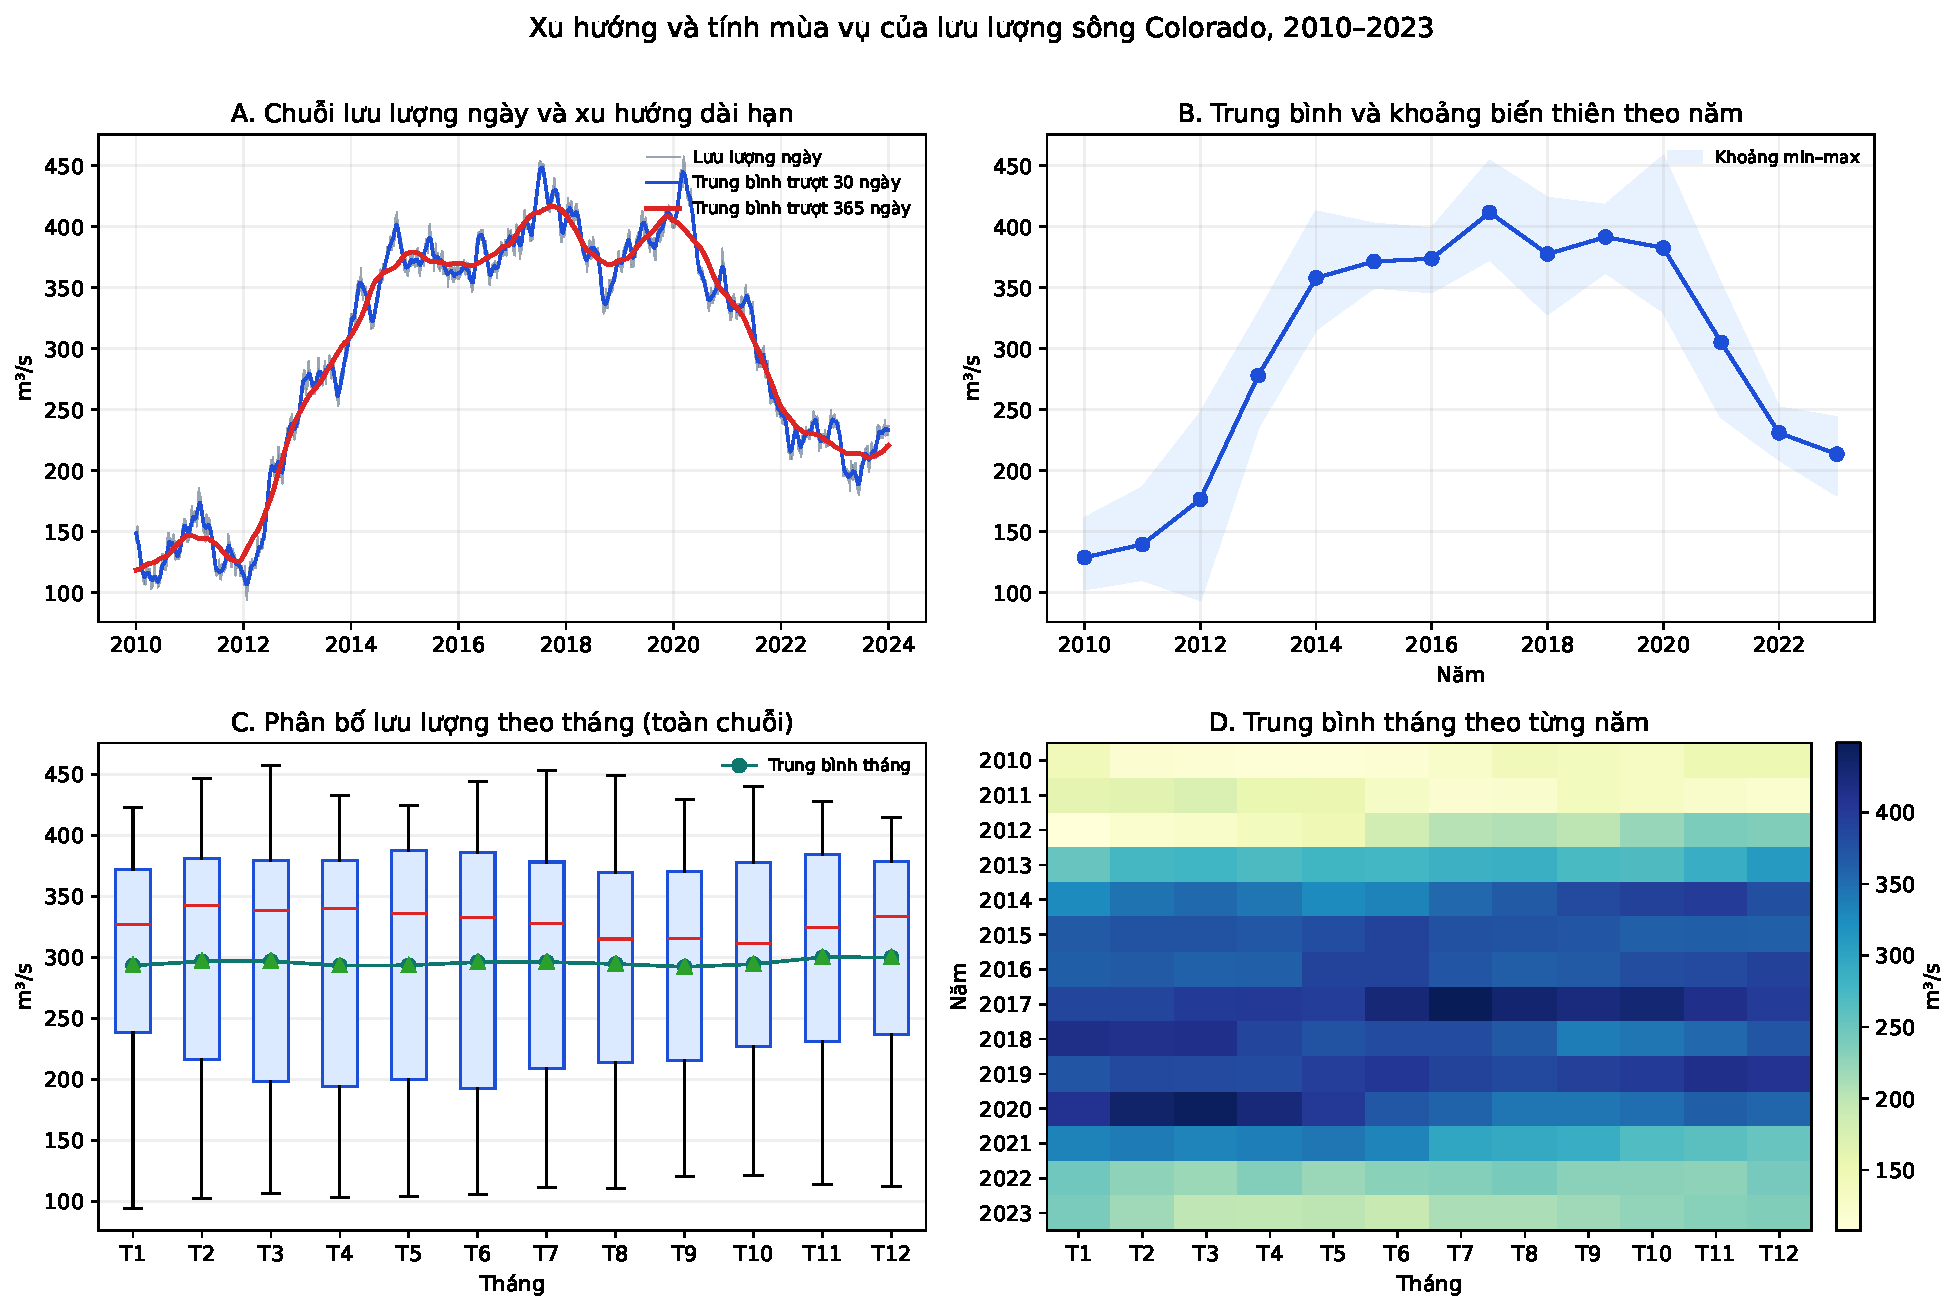
\includegraphics[width=0.86\linewidth]{figures/trend_seasonality.pdf}
\caption{Chuỗi lưu lượng ngày và thành phần xu hướng/mùa vụ. Mùa vụ gần như phẳng;
xu hướng thay đổi mạnh theo từng giai đoạn.}
\label{fig:q1}
\end{figure}

STL với chu kỳ 365 ngày và cấu hình robust cho seasonal strength \SeasonalStrength{}
và trend strength \TrendStrength. ACF lag 365 ngày là \AcfYear, rất gần 0; ACF lag 7
ngày và 30 ngày còn cao do tính liên tục ngắn hạn, không phải do mùa vụ năm. Vì vậy
không nên đọc chuỗi này như một mùa vụ đều đặn kiểu thủy văn ôn đới. Cần mô tả xu hướng
theo từng giai đoạn và nhấn mạnh các năm 2017--2019 có mức lưu lượng cao nổi bật.

\section{Câu hỏi 2: Các đợt lưu lượng cao}

Q95 toàn chuỗi là \QHigh{} m³/s. Có \NDaysHigh{} ngày vượt ngưỡng, chiếm \ShareHigh\%
chuỗi, gom thành \NEvents{} đợt liên tiếp. Đợt dài nhất kéo dài \LongestEvent{} ngày;
đỉnh lớn nhất trong các đợt là \MaxEventPeak{} m³/s, thuộc năm 2017. Việc gộp các ngày
liên tiếp giúp phân biệt một đợt kéo dài với nhiều dao động ngắn.

\begin{figure}[H]
\centering
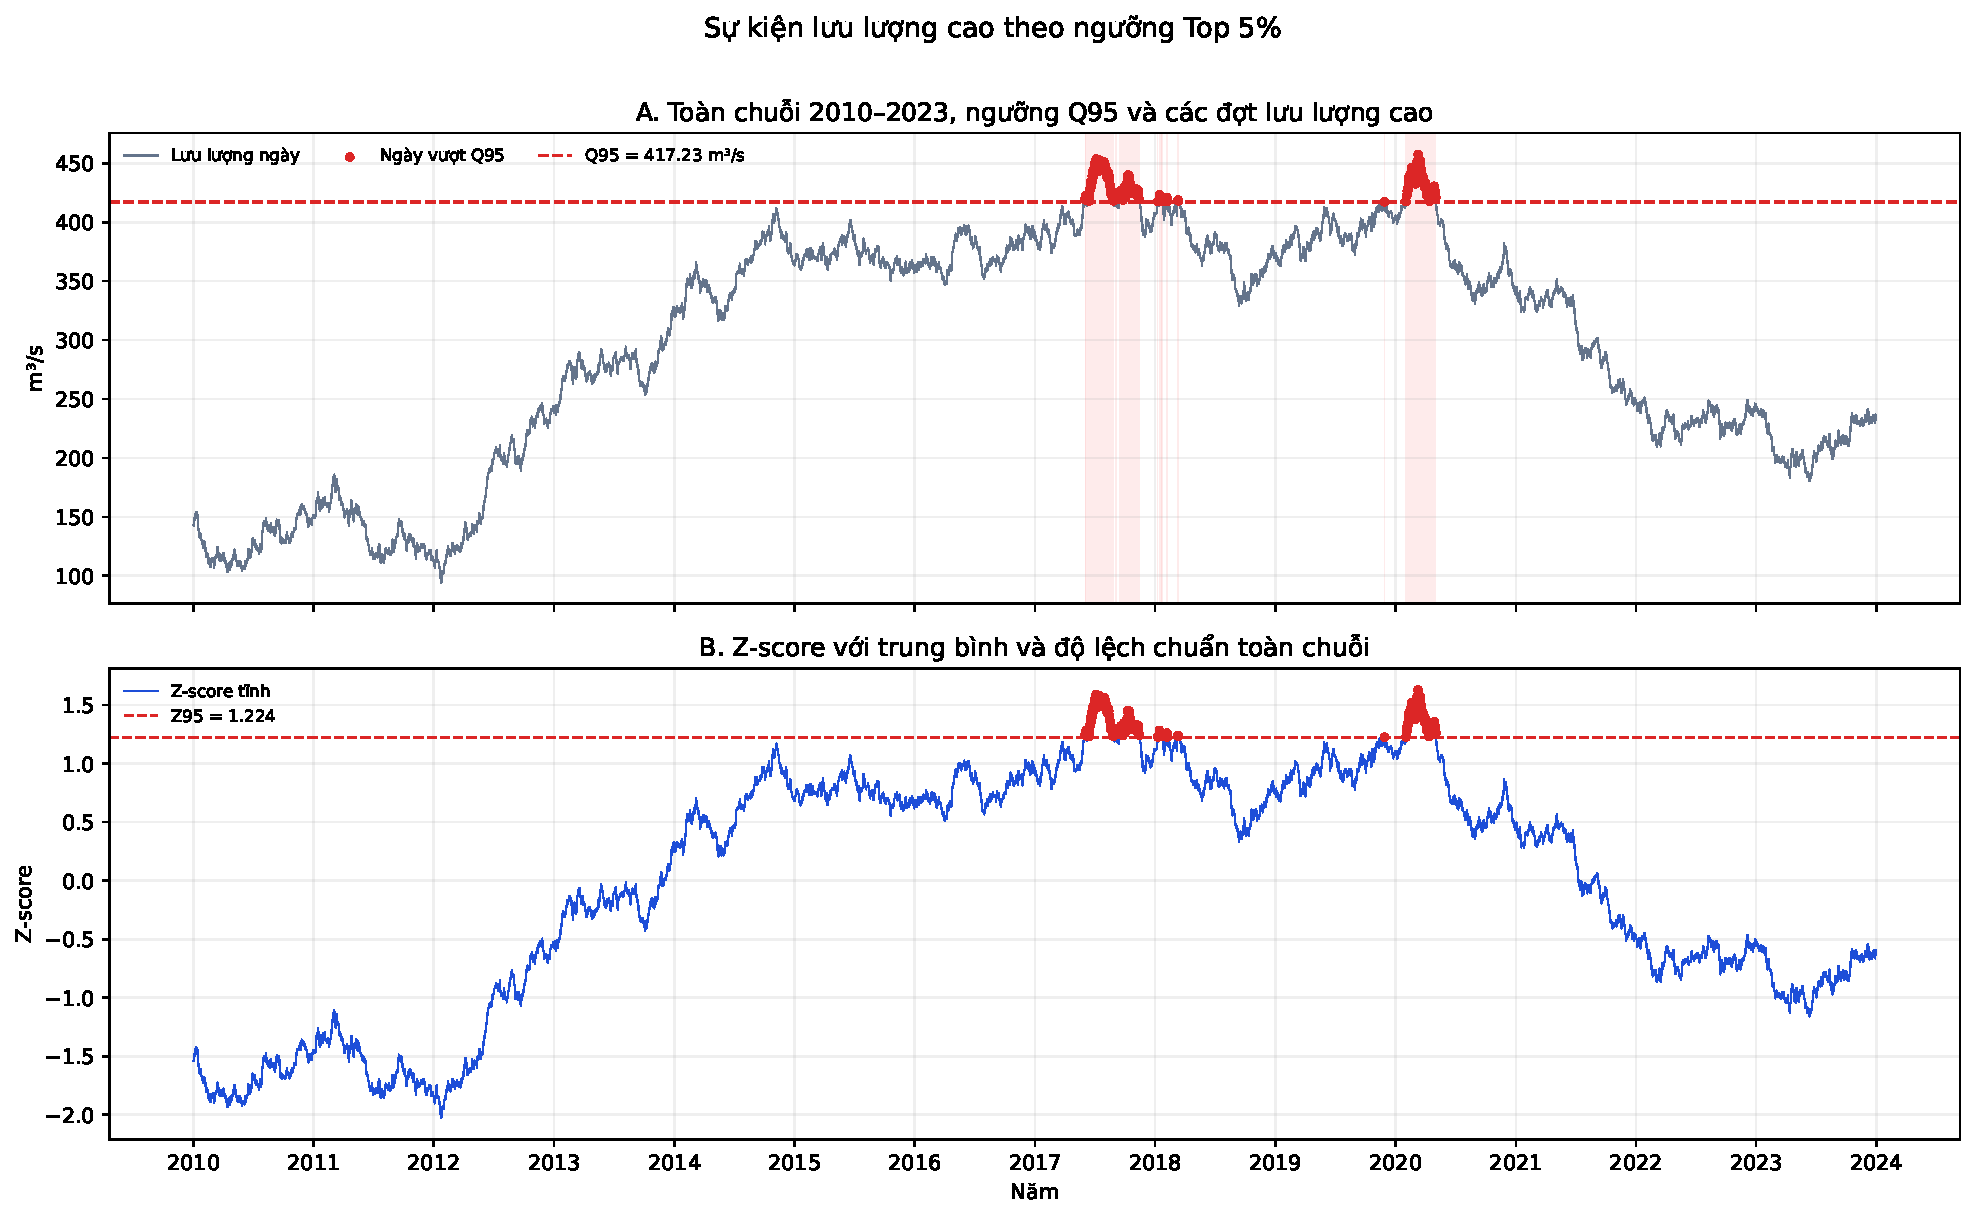
\includegraphics[width=0.86\linewidth]{figures/extremes_full_series.pdf}
\caption{Chuỗi lưu lượng và các ngày vượt Q95. Các đợt tập trung chủ yếu quanh
2017--2020.}
\label{fig:q2}
\end{figure}

\begin{table}[H]
\centering
\caption{Top 5 đợt theo đỉnh lưu lượng}
\label{tab:top5}
\small
\begin{tabular}{clrrr}
\toprule
Hạng & Khoảng ngày & Số ngày & Ngày đỉnh & Đỉnh (m³/s) \\
\midrule
1 & 04/02/2020–03/05/2020 & 90 & 10/03/2020 & 457{,}49 \\
2 & 13/06/2017–28/08/2017 & 77 & 06/07/2017 & 453{,}52 \\
3 & 15/09/2017–14/11/2017 & 61 & 11/10/2017 & 439{,}97 \\
4 & 02/09/2017–05/09/2017 & 4 & 03/09/2017 & 423{,}71 \\
5 & 13/01/2018–16/01/2018 & 4 & 14/01/2018 & 423{,}21 \\
\bottomrule
\end{tabular}

\end{table}

Bảng~\ref{tab:top5} cho thấy đợt dài nhất (90 ngày, đầu năm 2020) không phải đợt có
đỉnh lớn nhất; đỉnh lớn nhất nằm trong đợt tháng 6--8/2017. Vì ngưỡng Q95 tính trên
toàn chuỗi, số ngày vượt ngưỡng trong một năm cụ thể có thể cao hơn hoặc thấp hơn 5\%.
Kết quả này chỉ mô tả các đợt trong dữ liệu, không phải phân vùng rủi ro lũ.

\section{Câu hỏi 3: Dự báo 7 ngày}

Trên Validation, Naive persistence có mean RMSE 5,535 m³/s, LightGBM delta 5,569 m³/s
và Seasonal Naive 365 65,57 m³/s. LightGBM không vượt Naive một cách ổn định; early
stopping chọn số vòng lặp rất nhỏ ở một số horizon, cho thấy mô hình gần như quay về
persistence. Vì vậy kết quả được báo cáo nguyên trạng, không tinh chỉnh thêm trên Test.

\begin{table}[H]
\centering
\caption{Chỉ số trên Test 2022--2023 (724 ngày gốc, 5.068 cặp dự báo)}
\label{tab:metrics}
\small
\setlength{\tabcolsep}{3pt}
\begin{tabular}{lrrrrr}
\toprule
Mô hình & mean RMSE & mean MAE & mean NSE & pooled RMSE & pooled NSE \\
\midrule
Naive persistence & 5{,}31 & 4{,}16 & 0{,}881 & 5{,}50 & 0{,}882 \\
Seasonal Naive 365 & 60{,}48 & 46{,}45 & -13{,}333 & 60{,}48 & -13{,}333 \\
LightGBM direct 7 (delta) & 5{,}33 & 4{,}17 & 0{,}881 & 5{,}52 & 0{,}881 \\
\bottomrule
\end{tabular}

\end{table}

Bảng~\ref{tab:metrics} cho thấy Naive persistence có mean RMSE \NaiveMeanRmse{} m³/s,
thấp hơn LightGBM \LgbmMeanRmse{} m³/s một chút. Seasonal Naive 365 rất kém
(\SeasonalMeanRmse{} m³/s), phù hợp với kết luận mùa vụ yếu ở Q1. Với LightGBM, D+1 có
RMSE 2,79 m³/s và NSE 0,970; D+7 có RMSE 7,10 m³/s và NSE 0,802. Naive cũng đi từ
2,79 m³/s ở D+1 lên 7,05 m³/s ở D+7. Sai số tăng theo horizon là hành vi hợp lý của
dự báo chuỗi thời gian.

\begin{figure}[H]
\centering
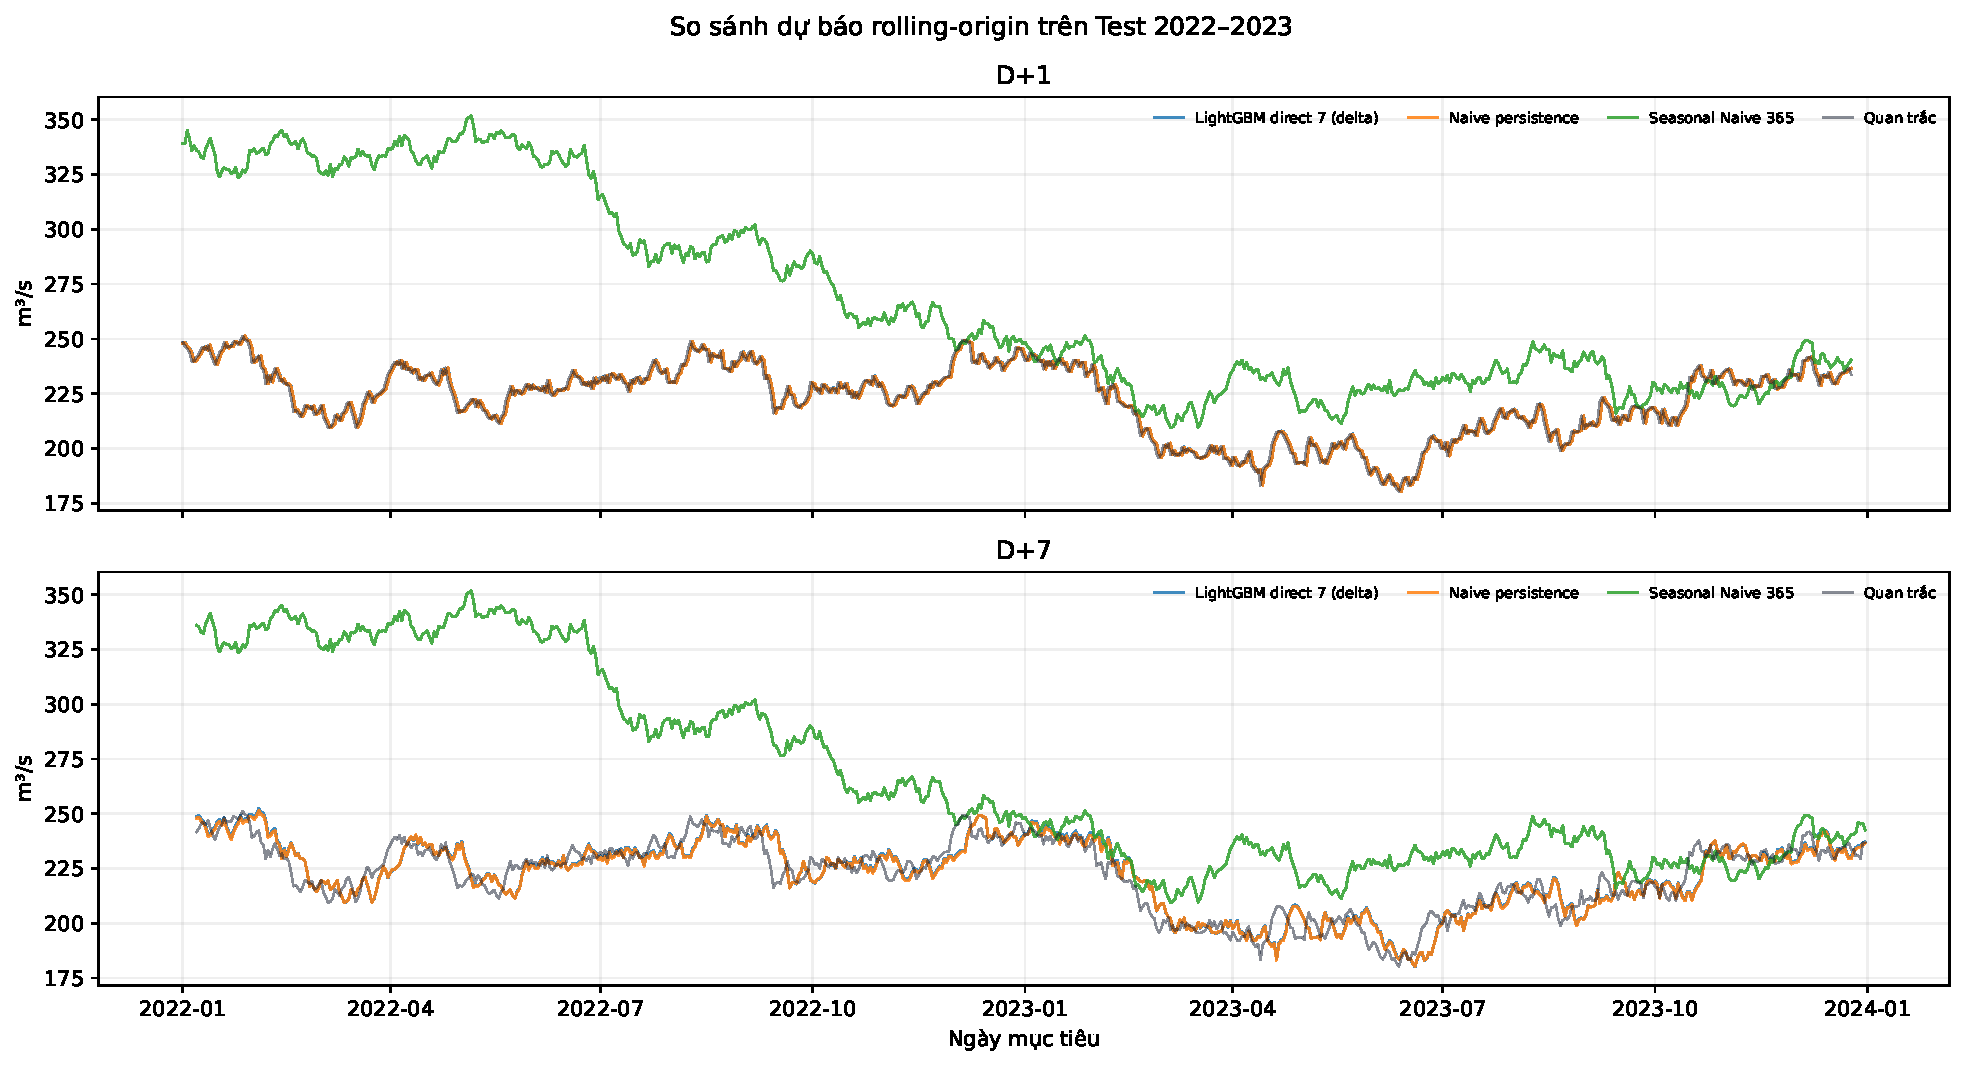
\includegraphics[width=0.84\linewidth]{figures/forecast_hydrograph.pdf}
\caption{Backtest 7 ngày: hai panel minh họa D+1 và D+7 với lịch sử, dự báo và giá trị
thực tế. Đường dự báo gần như bám mức persistence khi mô hình không tìm thấy tín hiệu
vượt trội.}
\label{fig:forecast}
\end{figure}

Kết quả này không có nghĩa LightGBM vô dụng. Mô hình vẫn học được cấu trúc phi tuyến
và đạt NSE cao, nhưng lợi thế so với persistence không ổn định trên Test. Với chuỗi
ngày có độ nhớt cao, baseline mạnh là đối thủ khó thay thế. Nếu mục tiêu là dự báo
vận hành, cần bổ sung biến ngoại sinh và đánh giá dài hạn hơn.

\section{Thảo luận và giới hạn}

Kết quả Q1--Q3 nhất quán với nhau: chuỗi có xu hướng dài hạn mạnh, mùa vụ yếu và các
đợt cực trị tập trung ở một số năm. Chính vì mùa vụ yếu, Seasonal Naive 365 thất bại
nặng; và vì chuỗi gần random-walk ở tần suất ngày, Naive persistence là baseline mạnh.

Các giới hạn chính:
\begin{itemize}
  \item Chỉ có 14 năm dữ liệu ngày; Test chỉ 2 năm, chưa đủ cho kết luận dài hạn.
  \item Chưa dùng biến ngoại sinh như mưa, nhiệt độ, tuyết tan hay vận hành hồ chứa.
  \item GRU chưa chạy trong môi trường hiện tại; báo cáo không có kết quả GRU.
  \item LightGBM dùng mục tiêu delta; đây là lựa chọn kỹ thuật đã ghi rõ, không phải
        kết quả được chọn theo Test.
  \item Đây là backtest, không phải dự báo vận hành hoặc cảnh báo lũ.
\end{itemize}

Về mặt phương pháp, việc giữ Test tách biệt và không tinh chỉnh trên Test là điều kiện
cần để kết quả có ý nghĩa. Việc Naive thắng LightGBM một chút là kết quả trung thực,
không phải lỗi cần che giấu. Nếu tiếp tục phát triển, nên thử mô hình có biến ngoại
sinh, kiểm định rolling-origin dài hơn và phân tích sai số theo mùa.

\section{Kết luận}

Chuỗi lưu lượng sông Colorado 2010--2023 có biến thiên năm lớn hơn nhiều so với mùa vụ
trung bình. Q95 toàn chuỗi là \QHigh{} m³/s, với \NDaysHigh{} ngày vượt ngưỡng trong
\NEvents{} đợt. Trên Test 2022--2023, Naive persistence đạt mean RMSE \NaiveMeanRmse{}
m³/s, nhỉnh hơn LightGBM direct 7 (\LgbmMeanRmse{} m³/s) một chút; Seasonal Naive 365
kém rõ rệt. Kết quả nhấn mạnh tầm quan trọng của baseline mạnh, chia tập theo thời gian
và báo cáo đúng phạm vi backtest.

\section*{Phụ lục A. Sai số theo từng horizon}

Bảng~\ref{tab:horizon} chi tiết hóa kết quả Test của Naive persistence và LightGBM
direct 7. Chạy lại pipeline với cấu hình trong mã nguồn và dữ liệu có mã băm bắt đầu
\texttt{\DatasetHashShort} sẽ tái tạo các giá trị này.

\begin{table}[H]
\centering
\caption{Sai số Test theo horizon (724 ngày gốc mỗi horizon)}
\label{tab:horizon}
\small
\begin{tabular}{crrrrrr}
\toprule
Horizon & \multicolumn{3}{c}{Naive persistence} & \multicolumn{3}{c}{LightGBM direct 7} \\
\cmidrule(lr){2-4}\cmidrule(lr){5-7}
 & RMSE & MAE & NSE & RMSE & MAE & NSE \\
\midrule
D+1 & 2{,}79 & 2{,}23 & 0{,}970 & 2{,}79 & 2{,}23 & 0{,}970 \\
D+2 & 3{,}93 & 3{,}12 & 0{,}940 & 3{,}93 & 3{,}12 & 0{,}940 \\
D+3 & 4{,}87 & 3{,}85 & 0{,}907 & 4{,}87 & 3{,}85 & 0{,}907 \\
D+4 & 5{,}60 & 4{,}42 & 0{,}877 & 5{,}60 & 4{,}43 & 0{,}877 \\
D+5 & 6{,}23 & 4{,}91 & 0{,}848 & 6{,}25 & 4{,}93 & 0{,}846 \\
D+6 & 6{,}68 & 5{,}16 & 0{,}824 & 6{,}72 & 5{,}19 & 0{,}822 \\
D+7 & 7{,}05 & 5{,}40 & 0{,}804 & 7{,}10 & 5{,}45 & 0{,}802 \\
\bottomrule
\end{tabular}

\end{table}

LightGBM chỉ nhỉnh hơn Naive ở D+1 (2,79 so với 2,79 m³/s sau làm tròn) và kém hơn
từ D+2 trở đi. Điều này cho thấy mô hình học máy chưa tạo được lợi thế ổn định so với
baseline persistence trên giai đoạn Test.

\section*{Phụ lục B. Hồ sơ số}

Mã nguồn, cấu hình, checkpoint, bảng kết quả và website tĩnh nằm trong
\texttt{submission.zip}; \texttt{source\_code.zip} chứa mã và test;
\texttt{latex\_overleaf.zip} chứa toàn bộ source LaTeX. Website chạy cục bộ theo
\texttt{README.md}; báo cáo không gắn URL công khai chưa được kiểm chứng. Run hiện tại:
\texttt{\RunId}; dữ liệu \texttt{\DatasetHashShort}; 14 test Python pass. PDF này được
tái tạo từ cùng nguồn và được kiểm tra còn 5 trang.

\begin{thebibliography}{9}
\small
\bibitem{hyndman2021}
Hyndman, R. J., \& Athanasopoulos, G. (2021).
\textit{Forecasting: Principles and Practice} (3rd ed.). OTexts.

\bibitem{cleveland1990}
Cleveland, R. B., Cleveland, W. S., McRae, J. E., \& Terpenning, I. (1990).
STL: A seasonal-trend decomposition procedure based on loess.
\textit{Journal of Official Statistics}, 6(1), 3--73.

\bibitem{ke2017}
Ke, G., Meng, Q., Finley, T., Wang, T., Chen, W., Ma, W., Ye, Q., \& Liu, T.-Y. (2017).
LightGBM: A highly efficient gradient boosting decision tree.
\textit{Advances in Neural Information Processing Systems}, 30.

\bibitem{pedregosa2011}
Pedregosa, F., et al. (2011).
Scikit-learn: Machine learning in Python.
\textit{Journal of Machine Learning Research}, 12, 2825--2830.
\end{thebibliography}


\end{document}
